\documentclass{ximera}

\usepackage{epsfig}

\graphicspath{
  {./}
  {figures/}
}


\usepackage{morewrites}

%\newcounter{ccounter}
%\setcounter{ccounter}{1}
%\newcommand{\Chapter}[1]{\setcounter{chapter}{\arabic{ccounter}}\chapter{#1}\addtocounter{ccounter}{1}}

%\newcommand{\section}[1]{\section{#1}\setcounter{thm}{0}\setcounter{equation}{0}}

%\renewcommand{\theequation}{\arabic{chapter}.\arabic{section}.\arabic{equation}}
%\renewcommand{\thefigure}{\arabic{chapter}.\arabic{figure}}
%\renewcommand{\thetable}{\arabic{chapter}.\arabic{table}}

%\newcommand{\Sec}[2]{\section{#1}\markright{\arabic{ccounter}.\arabic{section}.#2}\setcounter{equation}{0}\setcounter{thm}{0}\setcounter{figure}{0}}

\newcommand{\Sec}[2]{\section{#1}}

\setcounter{secnumdepth}{2}
%\setcounter{secnumdepth}{1} 

%\newcounter{THM}
%\renewcommand{\theTHM}{\arabic{chapter}.\arabic{section}}

\newcommand{\trademark}{{R\!\!\!\!\!\bigcirc}}
%\newtheorem{exercise}{}

\newcommand{\dfield}{{\sf dfield9}}
\newcommand{\pplane}{{\sf pplane9}}

\newcommand{\EXER}{\section*{Exercises}}%\vspace*{0.2in}\hrule\small\setcounter{exercise}{0}}
\newcommand{\CEXER}{}%\vspace{0.08in}\begin{center}Computer Exercises\end{center}}
\newcommand{\TEXER}{} %\vspace{0.08in}\begin{center}Hand Exercises\end{center}}
\newcommand{\AEXER}{} %\vspace{0.08in}\begin{center}Hand Exercises\end{center}}

% BADBAD: \newcommand{\Bbb}{\bf}

\newcommand{\R}{\mbox{$\Bbb{R}$}}
\newcommand{\C}{\mbox{$\Bbb{C}$}}
\newcommand{\Z}{\mbox{$\Bbb{Z}$}}
\newcommand{\N}{\mbox{$\Bbb{N}$}}
\newcommand{\D}{\mbox{{\bf D}}}
\usepackage{amssymb}
%\newcommand{\qed}{\hfill\mbox{\raggedright$\square$} \vspace{1ex}}
%\newcommand{\proof}{\noindent {\bf Proof:} \hspace{0.1in}}

\newcommand{\setmin}{\;\mbox{--}\;}
\newcommand{\Matlab}{{M\small{AT\-LAB}} }
\newcommand{\Matlabp}{{M\small{AT\-LAB}}}
\newcommand{\computer}{\Matlab Instructions}
\newcommand{\half}{\mbox{$\frac{1}{2}$}}
\newcommand{\compose}{\raisebox{.15ex}{\mbox{{\scriptsize$\circ$}}}}
\newcommand{\AND}{\quad\mbox{and}\quad}
\newcommand{\vect}[2]{\left(\begin{array}{c} #1_1 \\ \vdots \\
 #1_{#2}\end{array}\right)}
\newcommand{\mattwo}[4]{\left(\begin{array}{rr} #1 & #2\\ #3
&#4\end{array}\right)}
\newcommand{\mattwoc}[4]{\left(\begin{array}{cc} #1 & #2\\ #3
&#4\end{array}\right)}
\newcommand{\vectwo}[2]{\left(\begin{array}{r} #1 \\ #2\end{array}\right)}
\newcommand{\vectwoc}[2]{\left(\begin{array}{c} #1 \\ #2\end{array}\right)}



\newcommand{\inv}{^{-1}}
\newcommand{\CC}{{\cal C}}
\newcommand{\CCone}{\CC^1}
\newcommand{\Span}{{\rm span}}
\newcommand{\rank}{{\rm rank}}
\newcommand{\trace}{{\rm tr}}
\newcommand{\RE}{{\rm Re}}
\newcommand{\IM}{{\rm Im}}
\newcommand{\nulls}{{\rm null\;space}}

\newcommand{\dps}{\displaystyle}
\newcommand{\arraystart}{\renewcommand{\arraystretch}{1.8}}
\newcommand{\arrayfinish}{\renewcommand{\arraystretch}{1.2}}
\newcommand{\Start}[1]{\vspace{0.08in}\noindent {\bf Section~\ref{#1}}}
\newcommand{\exer}[1]{\noindent {\bf \ref{#1}}}
\newcommand{\ans}{}
\newcommand{\matthree}[9]{\left(\begin{array}{rrr} #1 & #2 & #3 \\ #4 & #5 & #6
\\ #7 & #8 & #9\end{array}\right)}
\newcommand{\cvectwo}[2]{\left(\begin{array}{c} #1 \\ #2\end{array}\right)}
\newcommand{\cmatthree}[9]{\left(\begin{array}{ccc} #1 & #2 & #3 \\ #4 & #5 &
#6 \\ #7 & #8 & #9\end{array}\right)}
\newcommand{\vecthree}[3]{\left(\begin{array}{r} #1 \\ #2 \\
#3\end{array}\right)}
\newcommand{\cvecthree}[3]{\left(\begin{array}{c} #1 \\ #2 \\
#3\end{array}\right)}
\newcommand{\cmattwo}[4]{\left(\begin{array}{cc} #1 & #2\\ #3
&#4\end{array}\right)}

\newcommand{\Matrix}[1]{\ensuremath{\left(\begin{array}{rrrrrrrrrrrrrrrrrr} #1 \end{array}\right)}}

\newcommand{\Matrixc}[1]{\ensuremath{\left(\begin{array}{cccccccccccc} #1 \end{array}\right)}}



\renewcommand{\labelenumi}{\theenumi)}
\newenvironment{enumeratea}%
{\begingroup
 \renewcommand{\theenumi}{\alph{enumi}}
 \renewcommand{\labelenumi}{(\theenumi)}
 \begin{enumerate}}
 {\end{enumerate}\endgroup}



\newcounter{help}
\renewcommand{\thehelp}{\thesection.\arabic{equation}}

%\newenvironment{equation*}%
%{\renewcommand\endequation{\eqno (\theequation)* $$}%
%   \begin{equation}}%
%   {\end{equation}\renewcommand\endequation{\eqno \@eqnnum
%$$\global\@ignoretrue}}

%\input{psfig.tex}

\author{Martin Golubitsky and Michael Dellnitz}

%\newenvironment{matlabEquation}%
%{\renewcommand\endequation{\eqno (\theequation*) $$}%
%   \begin{equation}}%
%   {\end{equation}\renewcommand\endequation{\eqno \@eqnnum
% $$\global\@ignoretrue}}

\newcommand{\soln}{\textbf{Solution:} }
\newcommand{\exercap}[1]{\centerline{Figure~\ref{#1}}}
\newcommand{\exercaptwo}[1]{\centerline{Figure~\ref{#1}a\hspace{2.1in}
Figure~\ref{#1}b}}
\newcommand{\exercapthree}[1]{\centerline{Figure~\ref{#1}a\hspace{1.2in}
Figure~\ref{#1}b\hspace{1.2in}Figure~\ref{#1}c}}
\newcommand{\para}{\hspace{0.4in}}

\renewenvironment{solution}{\suppress}{\endsuppress}

\ifxake
\newenvironment{matlabEquation}{\begin{equation}}{\end{equation}}
\else
\newenvironment{matlabEquation}%
{\let\oldtheequation\theequation\renewcommand{\theequation}{\oldtheequation*}\begin{equation}}%
  {\end{equation}\let\theequation\oldtheequation}
\fi

\makeatother


\title{mo11.tex}

\begin{document}
\begin{abstract}
BADBAD
\end{abstract}
\maketitle

\chapter{Autonomous Planar Nonlinear Systems}

\subsection*{Section~\protect{\ref{S:introAPNS}} Introduction}
\rhead{S:introAPNS}{INTRODUCTION}

\exer{c8.1.1}
There are 3 equilibria in the interval $[-3,1]$.  There are
asymptotically stable equilibria at $x\approx -2.910$ and at 
$x\approx 0.925$, and there is an asymptotically unstable equilibrium at
$x \approx -0.408$.  Figure~\ref{c8.1.1} shows the phase line
of the system.

\begin{figure}[htb]
                       \centerline{%
                       \psfig{file=exfigure/8-1-1.eps,width=3.5in}}
                \exercap{c8.1.1}
\end{figure}

\exer{c8.1.3a}
One valid initial condition is $X(0) = (1,4)$.  The {\tt y vs.\ t}
time series is shown in Figure~\ref{c8.1.3a}.

\exer{c8.1.3c} One valid initial condition is $X(0) = (1,2)$.  The
{\tt y vs.\ t} time series is shown in Figure~\ref{c8.1.3c}.

\para The trajectories in Exercises~\ref{c8.1.3a} and \ref{c8.1.3b} are
similar in backward time, since they limit on similar periodic
solutions as $t \rightarrow -\infty$.  Additionally, the trajectories
in \ref{c8.1.3a} and \ref{c8.1.3c} are similar in forward time, since
both approach infinity in the first quadrant.  In forward time,
\ref{c8.1.3b} approaches $y = 0$, and in backward time, \ref{c8.1.3c}
approaches $y = 0$.

\begin{figure}[htb]
                       \centerline{%
                       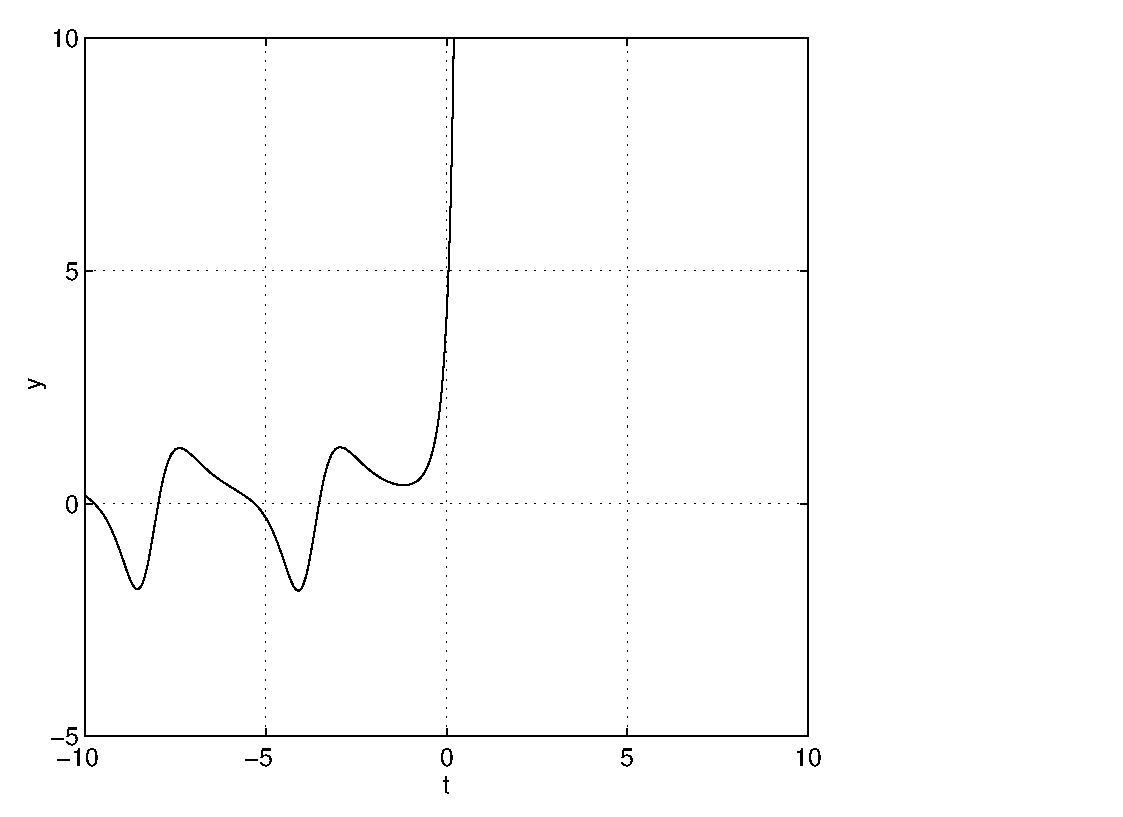
\psfig{file=exfigure/8-1-3a.eps,width=2.75in}
                       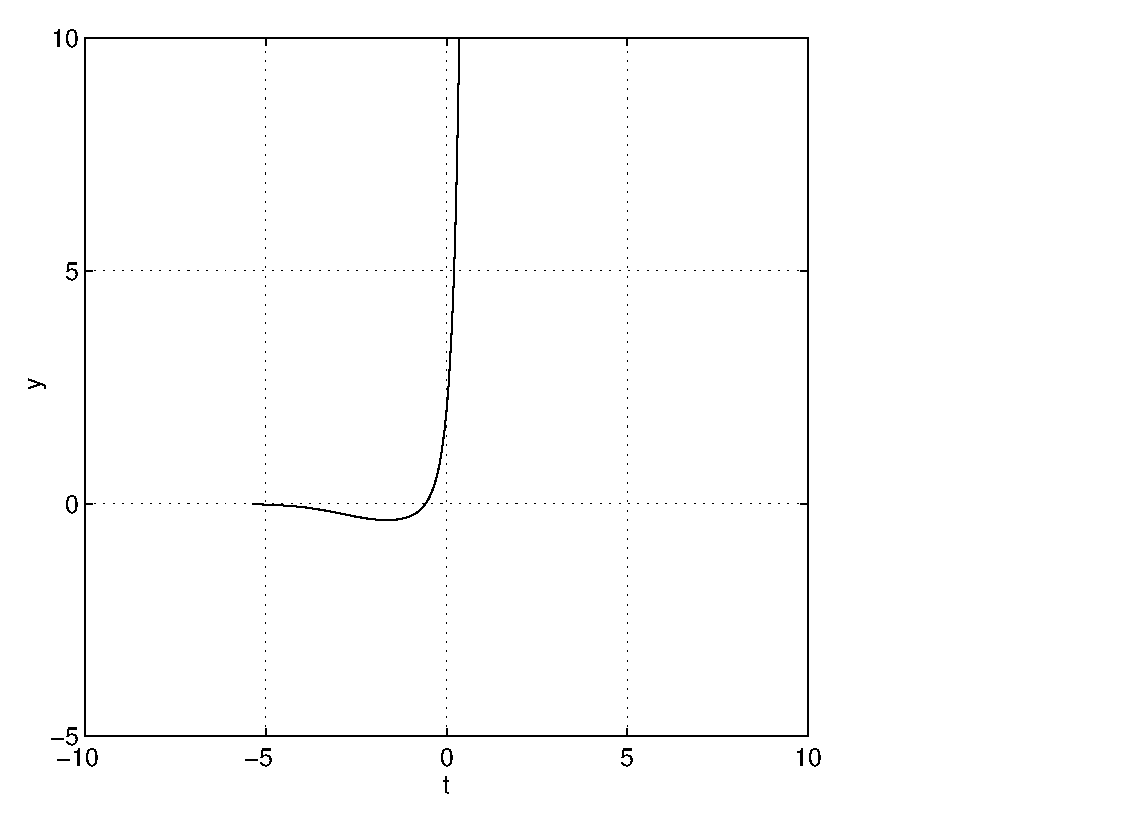
\psfig{file=exfigure/8-1-3c.eps,width=2.75in}}
		\centerline{Figure~\ref{c8.1.3a}\hspace{2.1in}
Figure~\ref{c8.1.3c}}
\end{figure}



\subsection*{Section~\protect{\ref{S:linearization}} Equilibria and Linearization}
\rhead{S:linearization}{EQUILIBRIA AND LINEARIZATION}

\exer{c8.2.1}
(a) \ans Figure~\ref{c8.2.1}a shows a phase line picture
of this system.

\soln There is a stable equilibrium at $x = 2$, and an unstable
equilibrium at $x = 1$, since $f(x) = -x^2 + 3x - 2 = (x - 1)(2 - x)$,
and since $f'(1) = 1 > 0$ and $f'(2) = -1 < 0$.

(b) \ans $\dps\lim_{t \to \infty} x(t) = -\infty$.

\soln The closest equilibrium to $x(0) = -1$ is $x = 1$, which is
unstable. 

(c) \ans Figure~\ref{c8.2.1}b shows the {\tt dfield5} graph of $y$.

\soln The trajectory of $y(t)$ with initial condition $y(0) = 0.5$ goes
to negative infinity in forward time, and limits on $y = 1$ in
backward time.

\begin{figure}[htb]
                       \centerline{%
                       \psfig{file=exfigure/8-2-1a.eps,width=2.75in}
                       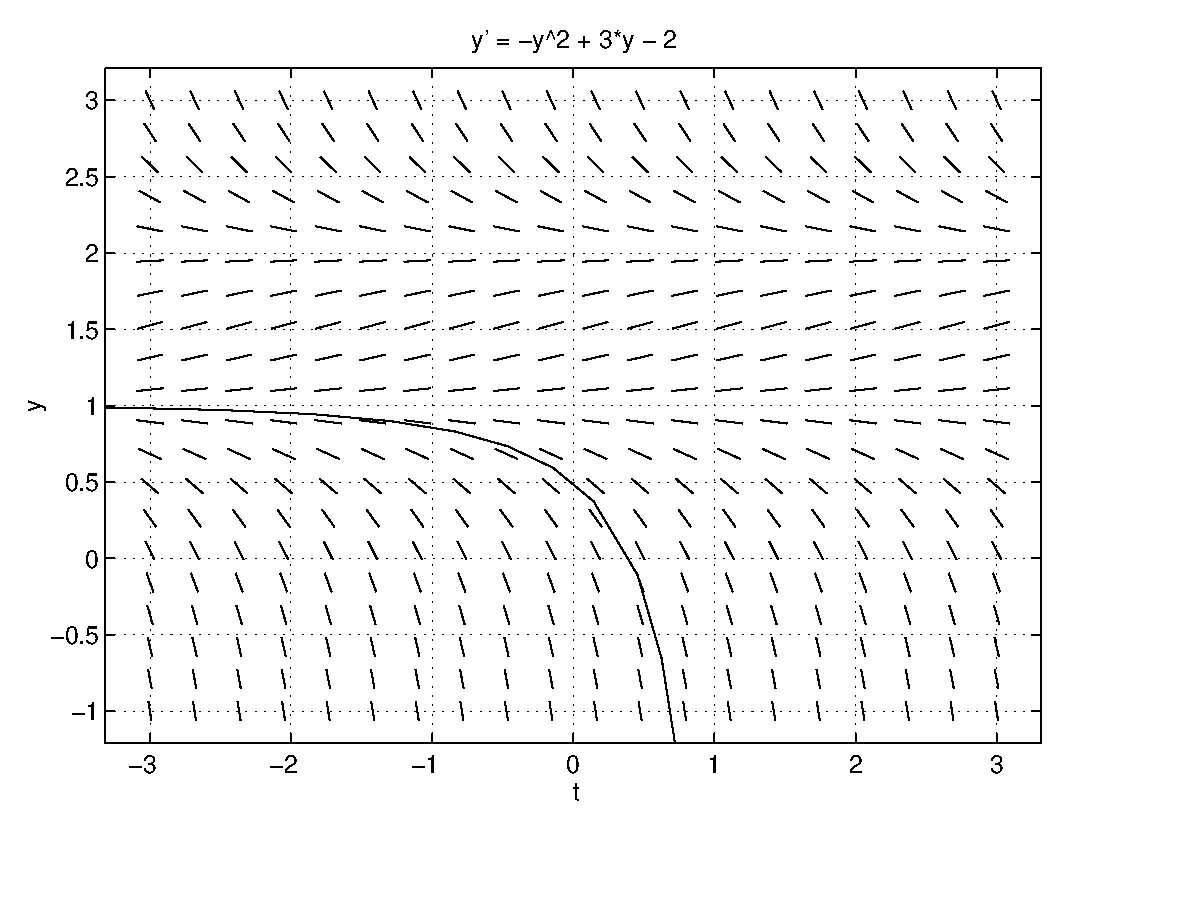
\psfig{file=exfigure/8-2-1b.eps,width=2.75in}}
                \exercaptwo{c8.2.1}
\end{figure}

\exer{c8.2.3}
(a) We are given $\frac{d\lambda}{dp} < 0$ for all $p$.  Thus $\lambda(p)$ is a 
monotonic decreasing function of $p$ when $p>0$ and the graph of 
$\lambda(p)$ can intersect $\lambda=0$ in at most one point.
Therefore, \Ref{E:pop} has at most one positive equilibrium.

(b) \ans If there exists a positive equilibrium $p_e$, then
$\dps\lim_{p \to \infty} p(t) = p_e$.  If no positive equilibrium
exists, then $\dps\lim_{p \to \infty} p(t) = \infty$.

\soln If there is a positive equilibrium, then it is asymptotically stable.
To verify this point differentiate the right hand side of \Ref{E:pop} with respect to 
$p$ and evaluate at $p=p_e$ obtaining
\[
\left.\frac{d}{dp}(\lambda(p)p)\right|_{p=p_e} = 
\lambda(p_e) + \lambda'(p_e)p_e = \lambda'(p_e)p_e <0
\]
since $\lambda(p_e) = 0$, $\lambda'(p_e) < 0$, and $p_e > 0$.  
So $p = p_e$ is a stable equilibrium, and the population limits on
$p_e$.

\para If no positive equilibrium exists, then $p = 0$, which is unstable,
is the only equilibrium, and the population grows without bound.

(c) Exercise~\ref{E:popex} is a specific example of \Ref{E:pop} in
which a positive equilibrium exists at $p = \frac{\lambda_0}{a}$.

\exer{c8.2.4b} \ans The origin is a spiral source.

\soln In this case, $\trace(C) = 9$ and $\det(C) = 22$, so the origin
is a hyperbolic equilibrium and a source.  Since the discriminant is 
$-1<0$, the origin is a spiral.

\exer{c8.2.4d} \ans The origin is not hyperbolic.

\soln Since $\det(C) = 0$ the origin is not hyperbolic.

\exer{c8.2.5}
(a) \ans The equilibria occur at $(x,y) = (1,0)$ and $(x,y) = (0,1)$.

\soln Solve $\frac{dx}{dt} = \frac{dy}{dt} = 0$.

(b) \ans The point $(x,y) = (1,0)$ is a saddle.  The point $(x,y) = (0,1)$
is a spiral sink.

\soln Let $f(x,y) = 1 - x - y$, $g(x,y) = 2xy$,
and $F = (f,g)$.  Then the Jacobian matrix is
\[
(dF)_{(x,y)} = \mattwo{f_x(x,y)}{f_y(x,y)}{g_x(x,y)}{g_y(x,y)}
= \mattwo{-1}{-1}{2y}{2x}.
\]
Specifically, at the equilibrium points:
\[
(dF)_{(1,0)} = \mattwo{-1}{-1}{0}{2} \qquad
(dF)_{(0,1)} = \mattwo{-1}{-1}{2}{0}.
\]
The eigenvalues of $(dF)_{(1,0)}$ are $\lambda_1 = 2$ and $\lambda_2 = -1$;
so the point is like a saddle in a small neighborhood.  The trace of
$(dF)_{(0,1)}$ is $-1 < 0$ and the determinant is $2 > 0$, so the
discriminant is negative and, within a small neighborhood, the point
is like a spiral sink.

(c) Compute the eigenvectors of the Jacobian of the saddle point $(1,0)$.
The invariant axes of $(1,0)$ are the eigendirections $(1,-3)$ and
$(1,0)$.  Use these vectors to graph the system.  Your sketch should
resemble the {\tt pplane5} graph in Figure~\ref{c8.2.5}.

\begin{figure}[htb]
                       \centerline{%
                       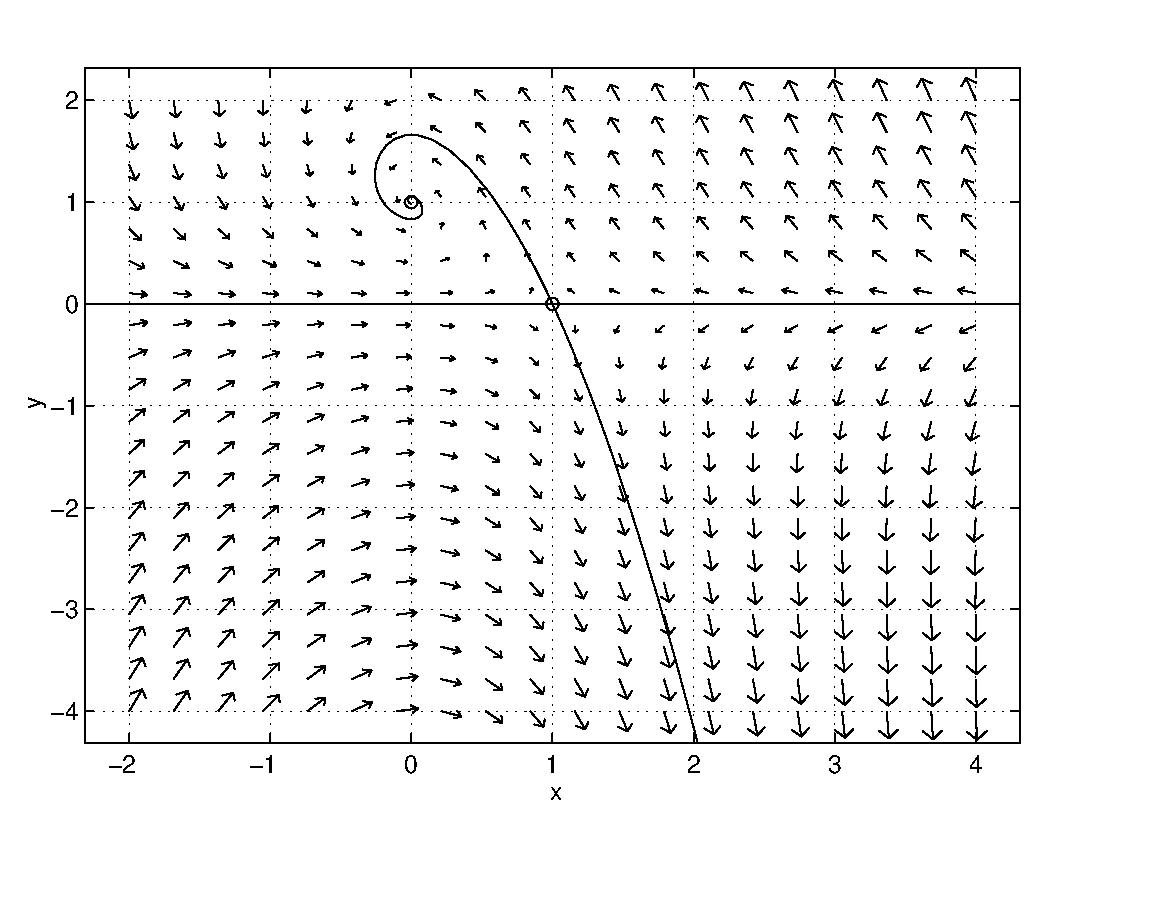
\psfig{file=exfigure/8-2-5.eps,width=3.0in}}
                \exercap{c8.2.5}
\end{figure}

\exer{c8.2.7}
(a) Solving system \Ref{e:global2exam} for $\dot{x} = \dot{y} = 0$
yields equilibria at $(0,0)$, $(\sqrt{2.2},0)$, and $(-\sqrt{2.2},0)$.

(b) The general Jacobian matrix for \Ref{e:global2exam} is
\[
(dJ)_{(x,y)} = \cmattwo{0}{1}{2.2 - 3x^2 + ay}{2.1 + ax}.
\]
The Jacobian matrices at the equilibria are:
\[ \begin{array}{rcl}
(dJ)_{(0,0)} & = & \cmattwo{0}{1}{2.2}{2.1} \\
(dJ)_{(\sqrt{2.2},0)} & = & \cmattwo{0}{1}{-4.4}{2.1 + \sqrt{2.2}a} \\
(dJ)_{(-\sqrt{2.2},0)} & = & \cmattwo{0}{1}{-4.4}{2.1 - \sqrt{2.2}a}. \\
\end{array}
\]

(c) \ans The Jacobian of the equilibrium at $(\sqrt{2.2},0)$ is not
hyperbolic at $a = -2.1\left/\sqrt{2.2}\right.$, and the Jacobian of the
equilibrium at $(-\sqrt{2.2},0)$ is not hyperbolic at
$a = 2.1\left/\sqrt{2.2}\right.$.

\soln Note that a matrix is nonhyperbolic if the determinant is positive
and the trace is zero.

(d) \ans The equilibrium at $(\sqrt{2.2},0)$ is asymptotically stable for
$a < -2.1\left/\sqrt{2.2}\right.$ and the equilibrium at
$(-\sqrt{2.2},0)$ is asymptotically stable for
$a > 2.1\left/\sqrt{2.2}\right.$.  Thus, there is no value of $a$ for which
both equilibria are stable.  The equilibrium at $(0,0)$ is not stable,
since the eigenvalues of the Jacobian have opposite sign.

\soln Note that the determinant of the Jacobian is always positive, so
the equilibria are stable for values of $a$ at which the trace is negative.

(e) For $a = -2.1/\sqrt{2.2}$, the equilibrium at $(\sqrt{2.2},0)$
is non-hyperbolic, with Jacobian matrix
\[
(dJ)_{(\sqrt{2.2},0)} = \mattwo{0}{1}{-4.4}{0}.
\]
The linear system $\dot{X} = (dJ)_{(\sqrt{2.2},0)}X$ is pictured in
Figure~\ref{c8.2.7}.  Note that the system is a center.  For
$a = 2.1/\sqrt{2.2}$, the equilibrium at $(-\sqrt{2.2},0)$ is
nonhyperbolic.  Its Jacobian at this point is identical to
$(dJ)_{(\sqrt{2.2},0)}$.

\begin{figure}[htb]
                       \centerline{%
                       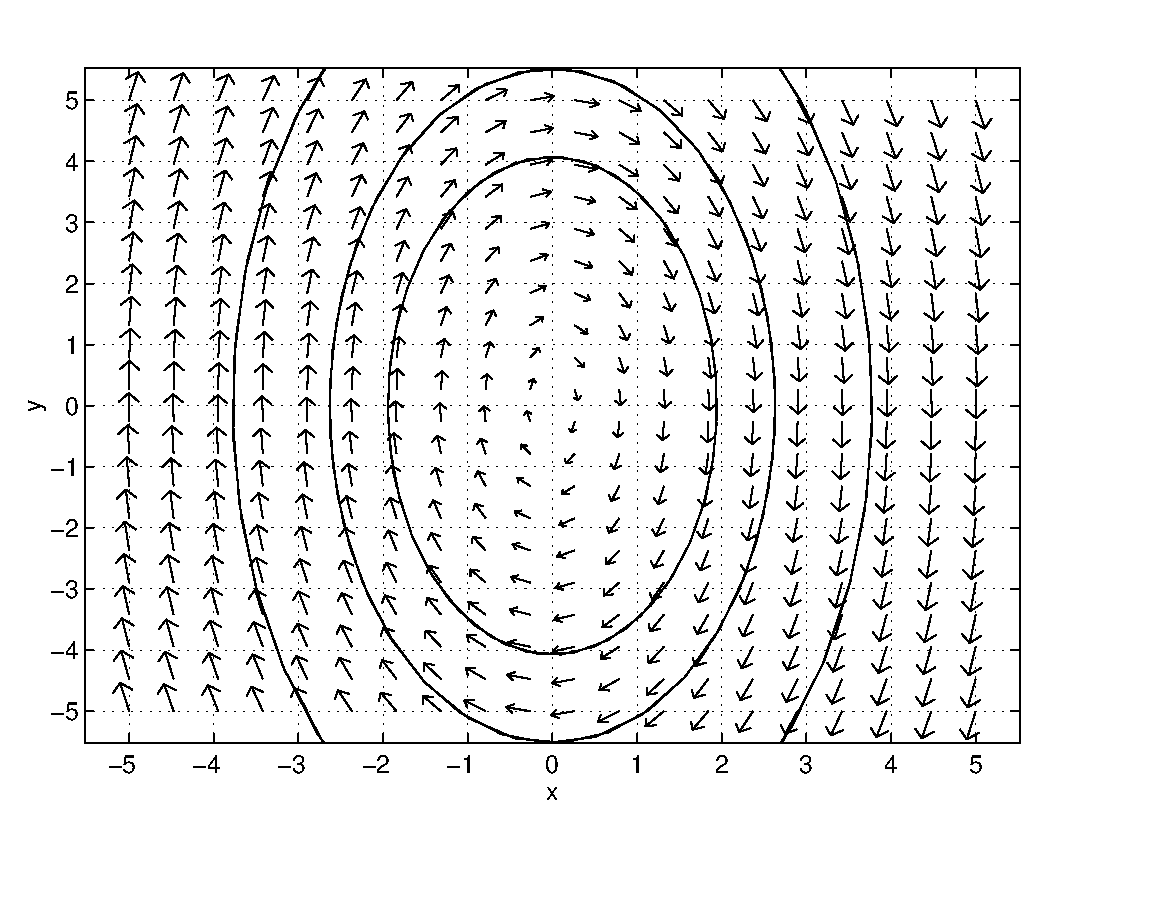
\psfig{file=exfigure/8-2-7.eps,width=3.0in}}
                \exercap{c8.2.7}
\end{figure}

\exer{E:nonhyp}
(a) Find all equilibria by computing $x$ and $y$ for $\dot{x} =
\dot{y} = 0$.  Then, from the second equation, $x = -y^3$, so
substituting into the first equation yields
\[
0 = y^9 + 2y^5 + y = y(y^4 + 1)^2.
\]
The only solution to this equation over the complex number system is
$y = 0$.  Therefore, the origin is the only equilibrium of
\Ref{e:nonhypcenter}.  The Jacobian matrix of \Ref{e:nonhypcenter} at
the origin is 
\[
(dJ)_{(0,0)} = \mattwo{0}{1}{-1}{0}.
\]
The eigenvalues of this Jacobian are $\pm i$.  Therefore, the equilibrium
is a center.

(b) First, compute $\dot{r}$:
\[
\frac{d}{dt}(r) = \frac{d}{dt}(\sqrt{x^2 + y^2}) =
\frac{1}{2\sqrt{x^2 + y^2}}\left(\frac{d}{dt}(x^2 + y^2)\right)
= \frac{1}{r}(x\dot{x} + y\dot{y}).
\]
Then, substitute \Ref{e:nonhypcenter} to obtain
\[
\dot{r} = \frac{1}{r}(x(y - x^3 - 2xy^2) + y(-x - y^3))
= -\frac{1}{r}(x^2 + y^2)^2 = -r^3.
\]
Note that $r''(t) = -3r(t)^2 < 0$.  Thus, $r = 0$ is a stable equilibrium
of \Ref{e:nonhypcenter}.

\exer{c8.2.11}
(a) The {\tt pplane5} command {\tt find an equilibrium} verifies this.

(b) {\tt pplane5} computes the eigenvectors as $v_1 = (0.4723,0.8814)$
(the eigenvector associated to $\lambda_1$) and $v_2 =
(0.9911,0.1328)$ (the eigenvector associated to $\lambda_2$).
Indeed, trajectories approach the origin in the direction of $v_2$.



\newpage
\subsection*{Section~\protect{\ref{S:periodic}} Periodic Solutions}
\rhead{S:periodic}{PERIODIC SOLUTIONS}

\exer{c8.3.1a}
\ans The system has two limit cycles, one at $r = 1$ and one at $r =
\sqrt{3}$, where $r$ is the radius of the circle made by the limit cycle.

\soln Write the differential equation in the form of \Ref{e:HopfNF}:
\[ \begin{array}{rcl}
\dot{x} & = & a(x^2 + y^2)x - b(x^2 + y^2)y \\
\dot{y} & = & a(x^2 + y^2)y + b(x^2 + y^2)x \end{array}
\]
where $a(r^2) = 3 - 4r^2 + r^4=(r^2-3)(r^2-1)$ and $b(r^2) = 5$.  Then,
rewrite the system in polar coordinates by calculating $\dot{r}$ and
$\dot{\theta}$ using \Ref{e:amplitude} and \Ref{e:phase} from the
chapter:
\[ \begin{array}{rcccl}
\dot{r} & = & a(r^2)r & = & (3 - 4r^2 + r^4)r \\
\dot{\theta} & = & b(r^2) & = & 5 \end{array}
\]
A limit cycle occurs at any positive equilibrium of $\frac{dr}{dt}$.
Solve for $r$ in the first equation to find that equilibria occur
at $r = 1$ and $r = \sqrt{3}$.  Then graph the system.  Your drawing
should resemble the {\tt pplane5} graph shown in Figure~\ref{c8.3.1a}.

\begin{figure}[htb]
                       \centerline{%
                       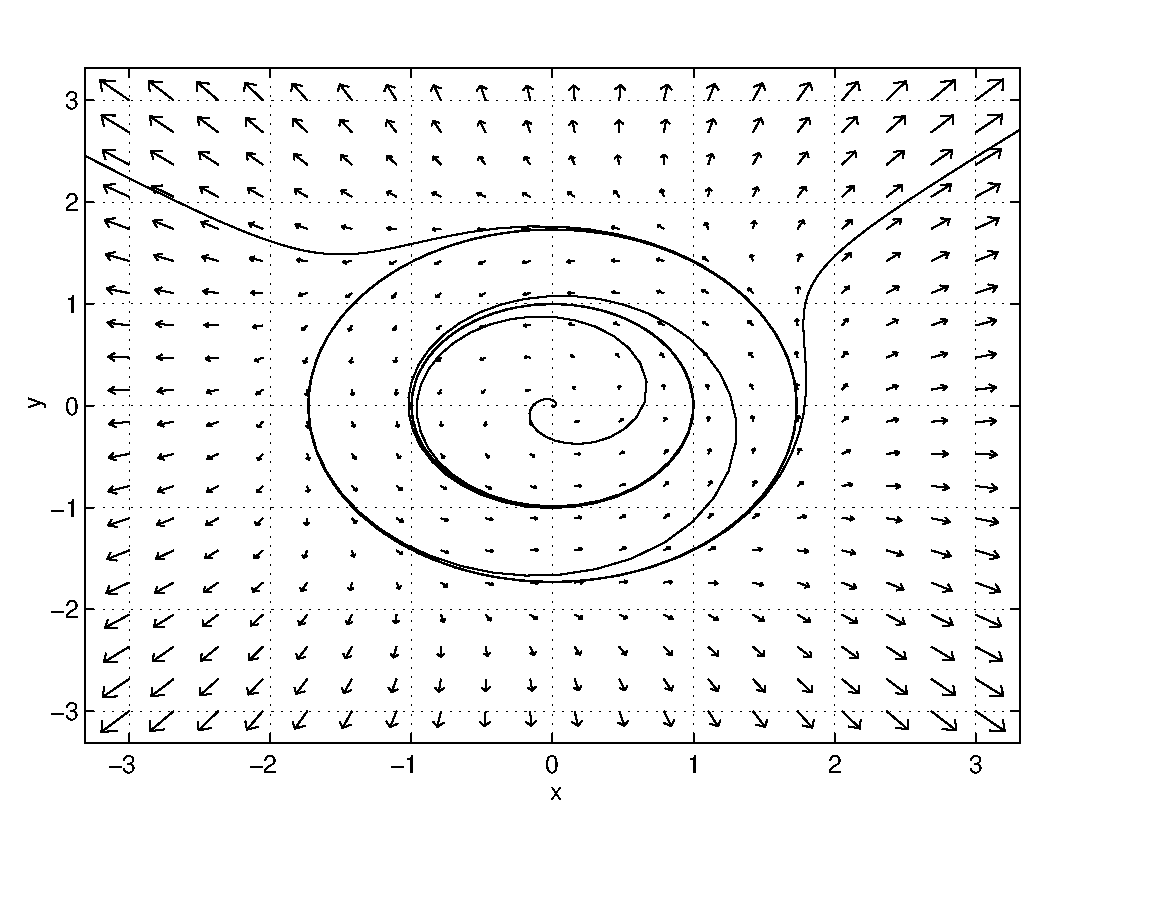
\psfig{file=exfigure/8-3-1.eps,width=3.0in}}
                \exercap{c8.3.1a}
\end{figure}

\exer{c8.3.1c}
\ans The system has two limit cycles, one at $r = \sqrt{2}$ and one
at $r = \sqrt{3}$. 

\soln Write the differential equation in the form of \Ref{e:HopfNF}
where $a(r^2) = 6 - 5r^2 + r^4=(r^2-3)(r^2-2)$, and 
$b(r^2) = 1+2r^2$.  Then,
rewrite the system in polar coordinates by calculating $\dot{r}$ and
$\dot{\theta}$ using \Ref{e:amplitude} and \Ref{e:phase} from the
chapter:
\[ 
\begin{array}{rcccl}
\dot{r} & = & a(r^2)r & = & (-5 + 4r^2 + r^4)r \\
\dot{\theta} & = & b(r^2) & = & 1+2r^2 \end{array}
\]
\newpage
A limit cycle occurs at any positive equilibrium of $\frac{dr}{dt}$.
Solve for $r$ in the first equation to find that a positive equilibrium 
occurs at $r = \sqrt{2}$ and $r = \sqrt{3}$.  Then graph the system.  Your 
drawing should resemble the {\tt pplane5} graph shown in Figure~\ref{c8.3.1c}.

\begin{figure}[htb]
                       \centerline{%
                       \psfig{file=exfigure/8-3-1c.eps,width=3.0in}}
                \exercap{c8.3.1c}
\end{figure}

\exer{c8.3.5}
\soln (a)  Use the chain rule to calculate
\[
\dot{h} = f_x\dot{x}+f_y\dot{y}.
\]
Using the gradient system of differential equations, observe that
\[
\dot{h} = f_x^2 + f_y^2\ge 0.
\]
(b) It follows from (a) that $\dot{h}(t_0)=0$ if and only if 
$f_x(x(t_0),y(t_0))=0$ and $f_y(x(t_0),y(t_0))=0$.  That is, 
$\dot{h}(t_0)=0$ if and only if $(x(t_0),y(t_0))$ is an equilibrium for the
gradient system.

\noindent (c) It follows from (b) that $\dot{h}$ is nowhere zero on a
nonconstant solution and from (a) that $\dot{h}(t)>0$ on a nonconstant
solution.  Therefore, $h(t)$ is monotonic increasing along any nonconstant
solution.

\noindent (d)  If $(x(t),y(t)$ is a nonconstant periodic solution of the
gradient system with period $T>0$, then $h(t+T)=h(t)$ for all $t$.  Thus,
$h(t)$ is not monotonic along this solution, contradicting (c).  Therefore,
nonconstant periodic solutions of gradient systems cannot exist.  

\exer{c8.3.3}
\ans There are nine equilibria in this square.

\soln  The equilibria found using {\sf pplane5} are:
\begin{verbatim}
(-0.7575, 0.3180)       Saddle point.            
(-1.9192, 0.0951)       Nodal source.            
(0.0000, 0.0000)        Spiral source.           
(1.9192, -0.0951)       Nodal source.            
(-0.7650, -1.2495)      Saddle point.            
(0.7650, 1.2495)        Saddle point.            
(0.7575, -0.3180)       Saddle point.            
(-0.1100, -2.6084)      Nodal source.            
(0.1100, 2.6084)        Nodal source.            
\end{verbatim}
See Figure~\ref{c8.3.3}.

\begin{figure}[htb]
                       \centerline{%
                       \psfig{file=exfigure/8-3-3.eps,width=3.0in}}
                \exercap{c8.3.3}
\end{figure}



\subsection*{Section~\protect{\ref{S:SPP}} Stylized Phase Portraits}
\rhead{S:SPP}{STYLIZED PHASE PORTRAITS}

\exer{c8.4.1}
Graph the system using {\tt pplane5}.  Then, find a saddle point at
$(-0.7426,-0.4902)$.  Plot the unstable and stable orbits.  The unstable
orbits and one stable orbit leave the graph window.  The other stable
orbit limits on a periodic solution around another equilibrium, the
spiral sink at $(-1.298,-3.209)$.  These are the only equilibria of
the system in this region.  The phase portrait is shown in
Figure~\ref{c8.4.1}.

\begin{figure}[htb]
                       \centerline{%
                       \psfig{file=exfigure/8-4-1.eps,width=3.0in}}
                \exercap{c8.4.1}
\end{figure}

\exer{c8.4.3}
The equilibria and their types are:
\begin{verbatim}
(1.4650, 1.3590)        Spiral source.           
(-1.3651, -1.4635)      Spiral sink.             
(1.4650, -1.3590)       Saddle point.            
(-1.3651, 1.4635)       Saddle point. 
\end{verbatim}
There are two limit cycles: one surrounding the spiral source at
$(1.4650, 1.3590)$ and one surrounding the spiral sink at $(-1.3651, -1.4635)$.

(a) A graph of the system is shown in Figure~\ref{c8.4.3}a.

(b) The four equilibria surround a roughly rectangular region.  As shown
by the connecting trajectories in the graph, all trajectories with
initial points inside this region remain in this region.  Note that this
includes trajectories with initial conditions inside the limit cycles.
All trajectories outside this region leave the window
$-3 \leq x,y \leq 3$ in forward or backward time.

(c) The {\tt pplane5} time series for the solution starting at $(0,0)$ is
shown in Figure~\ref{c8.4.3}b.

\begin{figure}[htb]
                       \centerline{%
                       \psfig{file=exfigure/8-4-3a.eps,width=2.75in}
                       \psfig{file=exfigure/8-4-3b.eps,width=2.75in}}
                \exercaptwo{c8.4.3}
\end{figure}

\exer{c8.4.5a}
\ans There are five equilibria and two limit cycles.  The phase portrait is
given in Figure~\ref{c8.4.5a}a.  The orbits that stay bounded in
forward time are indicated in Figure~\ref{c8.4.5a}b.

\soln (a)  Using {\sf pplane5} we can find five equilibria
\begin{verbatim}
(0.0000, 0.0000)        Spiral source.           
(1.8519, 1.2300)        Nodal source.            
(0.3445, 0.0485)        Saddle point.            
(0.3102, -0.1118)       Spiral sink.             
(0.0000, -0.3333)       Saddle point.            
\end{verbatim}
We can show that there are at most five equilibria by solving:
\begin{eqnarray*}
0.04x - y - 3y^2 + 2.5xy & = & 0\\
x - 3x^2 + 2x^2y & = & 0.
\end{eqnarray*}  
Factoring the second equation leads to 
\[
x=0 \quad \mbox{ or } \quad x = \frac{1}{3-2y}.
\]
Substituting $x=0$ into the first equation leads to the equilibria
$(0,0)$ and $(0,-\frac{1}{3})$. Substituting $x = \frac{1}{3-2y}$ into the
first equation yields
\[
\frac{0.04+2.5y}{3-2y} -(y+3y^2)=0.
\]
Multiplying this equation by $3-2y$ leads to a cubic equation that has at most
three roots.  Thus there are at most five equilibria in this system of
differential equations.

\noindent (b) There is numerical evidence for two limit cycles
one surrounding the spiral source at the origin and one surrounding the
spiral sink at $(0.3102, -0.1118)$.

\noindent (c)  The five equilibria, two limit cycles, and the stable and
unstable orbits of saddles are shown in Figure~\ref{c8.4.5a}a.

\noindent (d)  The solutions that stay bounded in forward time include the
equilibria, limit cycle and those indicated in Figure~\ref{c8.4.5a}b.

\begin{figure}[htb]
                       \centerline{%
                        \psfig{file=exfigure/8-4-5a.eps,width=2.75in}
			\psfig{file=exfigure/8-4-5a2.eps,width=2.75in}}
                \exercaptwo{c8.4.5a}
\end{figure}


\end{document}
